\chapter{2D Nominal Monte-Carlo Distributions, 2017}
\label{chap:nominal_mc_2017}
This chapter presents on the two dimensional \pmu \cosmu distributions for each selection present in the 2017 analysis. The simulated distributions use the prior central value and is referred to as the ``nominal''.

\section{FGD1 $\nu_\mu$ FHC}
\autoref{fig:nominal2D_FGD1numu} shows the \pmu \cosmu distributions and their ratios for FGD1, normalised to bin width. For FGD1 CC0$\pi$, the largest Data/MC discrepancies are in the very forward region around 500-1000 MeV/c, with some areas of low cross-section  (e.g. \pmu 2-5 GeV/c, \cosmu 0.85-0.9) mismodelled. The lines of constant $Q^2$ suggest high $Q^2$ behaviour is over-estimated in Monte-Carlo, whereas for $0.05 < Q^2 < 0.15 \text{ GeV}^2$ it is under-estimated. For CC1$\pi$ the most forward-goign bins are almost consistently under-estimated. As for CC0$\pi$, the $Q^2 >0.1 \text{GeV}^2$ region is over-estimated, but it is less clear at lower $Q^2$. For CCOther there is a band-like behaviour in $Q^2$ going from over estimation to underestimation up until $Q^2\sim0.1\text{ GeV}^2$. The high-momentum areas are mostly under-estimated in Monte-Carlo. It is also clear that ND280 are dominated by $0.05 < Q^2 < 0.30\text{ GeV}^2$ events.

\begin{figure}[h]
	\begin{subfigure}[t]{0.32\textwidth}
		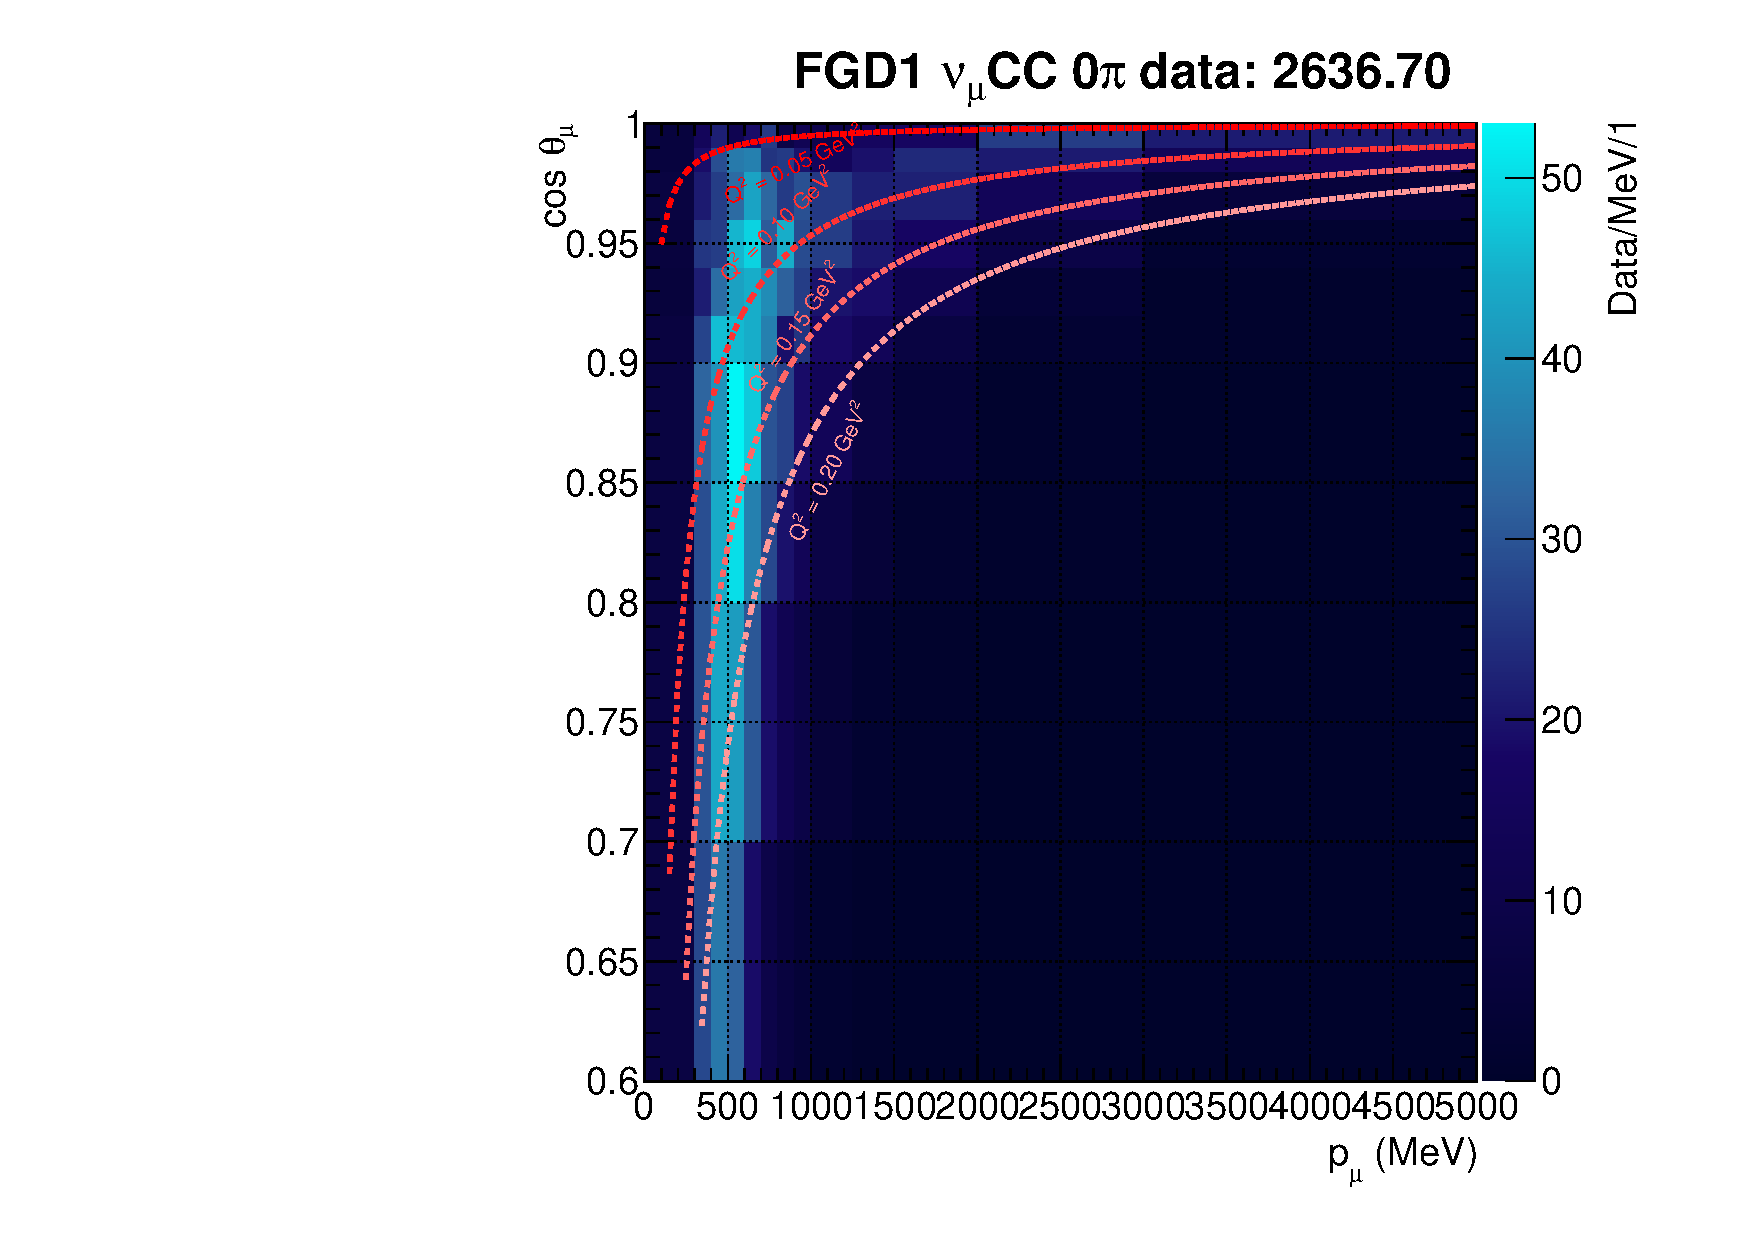
\includegraphics[width=\textwidth,page=1]{{figures/mach3/selection/2017b_nominal_withdebug_forthesis_ND280_nom.pdf}}
	\end{subfigure}
	\begin{subfigure}[t]{0.32\textwidth}
		\includegraphics[width=\textwidth,page=2]{{figures/mach3/selection/2017b_nominal_withdebug_forthesis_ND280_nom.pdf}}
	\end{subfigure}
	\begin{subfigure}[t]{0.32\textwidth}
		\includegraphics[width=\textwidth,page=3]{{figures/mach3/selection/2017b_nominal_withdebug_forthesis_ND280_nom.pdf}}
	\end{subfigure}
	
	\begin{subfigure}[t]{0.32\textwidth}
		\includegraphics[width=\textwidth,page=4]{{figures/mach3/selection/2017b_nominal_withdebug_forthesis_ND280_nom.pdf}}
	\end{subfigure}
	\begin{subfigure}[t]{0.32\textwidth}
		\includegraphics[width=\textwidth,page=5]{{figures/mach3/selection/2017b_nominal_withdebug_forthesis_ND280_nom.pdf}}
	\end{subfigure}
	\begin{subfigure}[t]{0.32\textwidth}
		\includegraphics[width=\textwidth,page=6]{{figures/mach3/selection/2017b_nominal_withdebug_forthesis_ND280_nom.pdf}}
	\end{subfigure}
	
	\begin{subfigure}[t]{0.32\textwidth}
		\includegraphics[width=\textwidth,page=7]{{figures/mach3/selection/2017b_nominal_withdebug_forthesis_ND280_nom.pdf}}
	\end{subfigure}
	\begin{subfigure}[t]{0.32\textwidth}
		\includegraphics[width=\textwidth,page=8]{{figures/mach3/selection/2017b_nominal_withdebug_forthesis_ND280_nom.pdf}}
	\end{subfigure}
	\begin{subfigure}[t]{0.32\textwidth}
		\includegraphics[width=\textwidth,page=9]{{figures/mach3/selection/2017b_nominal_withdebug_forthesis_ND280_nom.pdf}}
	\end{subfigure}
	
	\caption{Data and nominal MC distributions and the Data/MC ratio for FGD1 \numu selections. Lines of constant $Q^2_\text{reco}$ are shown. Bin content is normalised to bin width}
	\label{fig:nominal2D_FGD1numu}
\end{figure}

\section{FGD2 $\nu_\mu$ FHC}
\autoref{fig:nominal2D_FGD2numu} shows the same \numu selections for FGD2. The CC0$\pi$ selection is very similar to the FGD1 CC0$\pi$ selection, whereas the CC1$\pi$ selection appears better modelled for FGD2 than FGD1, although the opposite is true for CCOther.
\begin{figure}[h]
	\begin{subfigure}[t]{0.32\textwidth}
		\includegraphics[width=\textwidth,page=10]{{figures/mach3/selection/2017b_nominal_withdebug_forthesis_ND280_nom.pdf}}
	\end{subfigure}
	\begin{subfigure}[t]{0.32\textwidth}
		\includegraphics[width=\textwidth,page=11]{{figures/mach3/selection/2017b_nominal_withdebug_forthesis_ND280_nom.pdf}}
	\end{subfigure}
	\begin{subfigure}[t]{0.32\textwidth}
		\includegraphics[width=\textwidth,page=12]{{figures/mach3/selection/2017b_nominal_withdebug_forthesis_ND280_nom.pdf}}
	\end{subfigure}
	
	\begin{subfigure}[t]{0.32\textwidth}
		\includegraphics[width=\textwidth,page=13]{{figures/mach3/selection/2017b_nominal_withdebug_forthesis_ND280_nom.pdf}}
	\end{subfigure}
	\begin{subfigure}[t]{0.32\textwidth}
		\includegraphics[width=\textwidth,page=14]{{figures/mach3/selection/2017b_nominal_withdebug_forthesis_ND280_nom.pdf}}
	\end{subfigure}
	\begin{subfigure}[t]{0.32\textwidth}
		\includegraphics[width=\textwidth,page=15]{{figures/mach3/selection/2017b_nominal_withdebug_forthesis_ND280_nom.pdf}}
	\end{subfigure}
	
	\begin{subfigure}[t]{0.32\textwidth}
		\includegraphics[width=\textwidth,page=16]{{figures/mach3/selection/2017b_nominal_withdebug_forthesis_ND280_nom.pdf}}
	\end{subfigure}
	\begin{subfigure}[t]{0.32\textwidth}
		\includegraphics[width=\textwidth,page=17]{{figures/mach3/selection/2017b_nominal_withdebug_forthesis_ND280_nom.pdf}}
	\end{subfigure}
	\begin{subfigure}[t]{0.32\textwidth}
		\includegraphics[width=\textwidth,page=18]{{figures/mach3/selection/2017b_nominal_withdebug_forthesis_ND280_nom.pdf}}
	\end{subfigure}
	
	\caption{Data and nominal MC distributions and the Data/MC ratio for FGD2 \numu selections. Lines of constant $Q^2_\text{reco}$ are shown. Bin content is normalised to bin width}
	\label{fig:nominal2D_FGD2numu}
\end{figure}


\section{FGD1+2 $\bar{\nu}_\mu$ RHC}
\autoref{fig:nominal2D_FGD12numubar} shows the \pmu \cosmu for the \numubar selection, which again sees mostly consistent behaviour for the two FGDs for both the 1Track and NTracks selection. The event are mostly underestimated at low \pmu and become overestimated as we go up in \cosmu. The $Q^2$ bands appear present, notably in the 1 Track selections for $0.05 < Q^2 < 0.10 \text{ GeV}^2$.
\begin{figure}[h]
	\begin{subfigure}[t]{0.32\textwidth}
		\includegraphics[width=\textwidth,page=19]{{figures/mach3/selection/2017b_nominal_withdebug_forthesis_ND280_nom.pdf}}
	\end{subfigure}
	\begin{subfigure}[t]{0.32\textwidth}
		\includegraphics[width=\textwidth,page=20]{{figures/mach3/selection/2017b_nominal_withdebug_forthesis_ND280_nom.pdf}}
	\end{subfigure}
	\begin{subfigure}[t]{0.32\textwidth}
		\includegraphics[width=\textwidth,page=21]{{figures/mach3/selection/2017b_nominal_withdebug_forthesis_ND280_nom.pdf}}
	\end{subfigure}
	
	\begin{subfigure}[t]{0.32\textwidth}
		\includegraphics[width=\textwidth,page=22]{{figures/mach3/selection/2017b_nominal_withdebug_forthesis_ND280_nom.pdf}}
	\end{subfigure}
	\begin{subfigure}[t]{0.32\textwidth}
		\includegraphics[width=\textwidth,page=23]{{figures/mach3/selection/2017b_nominal_withdebug_forthesis_ND280_nom.pdf}}
	\end{subfigure}
	\begin{subfigure}[t]{0.32\textwidth}
		\includegraphics[width=\textwidth,page=24]{{figures/mach3/selection/2017b_nominal_withdebug_forthesis_ND280_nom.pdf}}
	\end{subfigure}
	
	\begin{subfigure}[t]{0.32\textwidth}
		\includegraphics[width=\textwidth,page=25]{{figures/mach3/selection/2017b_nominal_withdebug_forthesis_ND280_nom.pdf}}
	\end{subfigure}
	\begin{subfigure}[t]{0.32\textwidth}
		\includegraphics[width=\textwidth,page=26]{{figures/mach3/selection/2017b_nominal_withdebug_forthesis_ND280_nom.pdf}}
	\end{subfigure}
	\begin{subfigure}[t]{0.32\textwidth}
		\includegraphics[width=\textwidth,page=27]{{figures/mach3/selection/2017b_nominal_withdebug_forthesis_ND280_nom.pdf}}
	\end{subfigure}
	
	\begin{subfigure}[t]{0.32\textwidth}
		\includegraphics[width=\textwidth,page=28]{{figures/mach3/selection/2017b_nominal_withdebug_forthesis_ND280_nom.pdf}}
	\end{subfigure}
	\begin{subfigure}[t]{0.32\textwidth}
		\includegraphics[width=\textwidth,page=29]{{figures/mach3/selection/2017b_nominal_withdebug_forthesis_ND280_nom.pdf}}
	\end{subfigure}
	\begin{subfigure}[t]{0.32\textwidth}
		\includegraphics[width=\textwidth,page=30]{{figures/mach3/selection/2017b_nominal_withdebug_forthesis_ND280_nom.pdf}}
	\end{subfigure}
	\caption{Data and nominal MC distributions and the Data/MC ratio for FGD1 and FGD2 \numubar selections. Lines of constant $Q^2_\text{reco}$ are shown. Bin content is normalised to bin width}
	\label{fig:nominal2D_FGD12numubar}
\end{figure}

\section{FGD1+2 $\nu_\mu$ RHC}
\autoref{fig:nominal2D_FGD12numubar} shows the \numu in RHC selections, which generally populate higher \pmu due to the \numu flux in RHC mode. The samples are also statistically small so are more prone to larger statistical fluctuations. The CC1Track selection appears to have a pattern of underestimation at low \pmu, following the $Q^2$ band to high \pmu and high \cosmu.
\begin{figure}[h]
	\begin{subfigure}[t]{0.32\textwidth}
		\includegraphics[width=\textwidth,page=31]{{figures/mach3/selection/2017b_nominal_withdebug_forthesis_ND280_nom.pdf}}
	\end{subfigure}
	\begin{subfigure}[t]{0.32\textwidth}
		\includegraphics[width=\textwidth,page=32]{{figures/mach3/selection/2017b_nominal_withdebug_forthesis_ND280_nom.pdf}}
	\end{subfigure}
	\begin{subfigure}[t]{0.32\textwidth}
		\includegraphics[width=\textwidth,page=33]{{figures/mach3/selection/2017b_nominal_withdebug_forthesis_ND280_nom.pdf}}
	\end{subfigure}
	
	\begin{subfigure}[t]{0.32\textwidth}
		\includegraphics[width=\textwidth,page=34]{{figures/mach3/selection/2017b_nominal_withdebug_forthesis_ND280_nom.pdf}}
	\end{subfigure}
	\begin{subfigure}[t]{0.32\textwidth}
		\includegraphics[width=\textwidth,page=35]{{figures/mach3/selection/2017b_nominal_withdebug_forthesis_ND280_nom.pdf}}
	\end{subfigure}
	\begin{subfigure}[t]{0.32\textwidth}
		\includegraphics[width=\textwidth,page=36]{{figures/mach3/selection/2017b_nominal_withdebug_forthesis_ND280_nom.pdf}}
	\end{subfigure}
	
	\begin{subfigure}[t]{0.32\textwidth}
		\includegraphics[width=\textwidth,page=37]{{figures/mach3/selection/2017b_nominal_withdebug_forthesis_ND280_nom.pdf}}
	\end{subfigure}
	\begin{subfigure}[t]{0.32\textwidth}
		\includegraphics[width=\textwidth,page=38]{{figures/mach3/selection/2017b_nominal_withdebug_forthesis_ND280_nom.pdf}}
	\end{subfigure}
	\begin{subfigure}[t]{0.32\textwidth}
		\includegraphics[width=\textwidth,page=39]{{figures/mach3/selection/2017b_nominal_withdebug_forthesis_ND280_nom.pdf}}
	\end{subfigure}
	
	\begin{subfigure}[t]{0.32\textwidth}
		\includegraphics[width=\textwidth,page=40]{{figures/mach3/selection/2017b_nominal_withdebug_forthesis_ND280_nom.pdf}}
	\end{subfigure}
	\begin{subfigure}[t]{0.32\textwidth}
		\includegraphics[width=\textwidth,page=41]{{figures/mach3/selection/2017b_nominal_withdebug_forthesis_ND280_nom.pdf}}
	\end{subfigure}
	\begin{subfigure}[t]{0.32\textwidth}
		\includegraphics[width=\textwidth,page=42]{{figures/mach3/selection/2017b_nominal_withdebug_forthesis_ND280_nom.pdf}}
	\end{subfigure}
	\caption{Data and nominal MC distributions and the Data/MC ratio for FGD1 and FGD2 \numu in RHC selections. Lines of constant $Q^2_\text{reco}$ are shown. Bin content is normalised to bin width}
	\label{fig:nominal2D_FGD12numurhc}
\end{figure}



% % % % % % % % % % % % % % % % % % % % % % % % % % % %
% % Here is the nominal _UNSCALED_ MC
\iffalse
The raw Monte-Carlo \pmu \cosmu event distributions with aforementioned binning is shown in \autoref{fig:nominal_mc2d} with the projections and by-mode distributions in \autoref{fig:nominal_mcpmu} and \autoref{fig:nominal_mccosmu}. The 2D plots include lines of constant $Q^2_{\text{reco}}$, for $E_\nu = 0.6 \text{ GeV}$, defined as the reconstructed (observed) $Q^2$:
\begin{equation}
Q^2_{\text{reco}} = -m^2_\mu + 2E_\nu \left( E_\mu-p_\mu\cos\theta_\mu \right)
\end{equation}
which if looking at constant $Q^2_{\text{reco}}$ surfaces with fixed $E_\nu$ leads to a simple update scheme of
\begin{equation}
\cos\theta_{\mu, 2} = \frac{\sqrt{p_{\mu,2}^2+m_{\mu,2}^2} - \sqrt{p_{\mu,1}^2+m_{\mu,1}^2}+p_{\mu,1}\cos\theta_{\mu,1}}{p_{\mu,2}}
\end{equation}
As expected from the neutrino flux at ND280 and neutrino interaction cross-sections, the CC0$\pi$ selection is an order of magnitude more populated than the other \numu selections. CC1$\pi$ and CCOther have similar statistics, and FGD1 generally has marginally more events than FGD2, owing to the reconstruction effects discussed in \autoref{sec:ND280:sel}. The \numubar CC1Track selections have similar statistics to \numu CC1$\pi$ and CCOther, a factor five higher than \numubar CCNTrack. The \numu in RHC selections have similar statistics to the \numubar CCNTrack and roughly the same for 1Track and NTrack. All the selections focus in on the $Q^2$ range of $0.1 < Q^2 < 0.5 \text{ GeV}^2$.
\begin{figure}[h]
	\begin{subfigure}[t]{0.32\textwidth}
		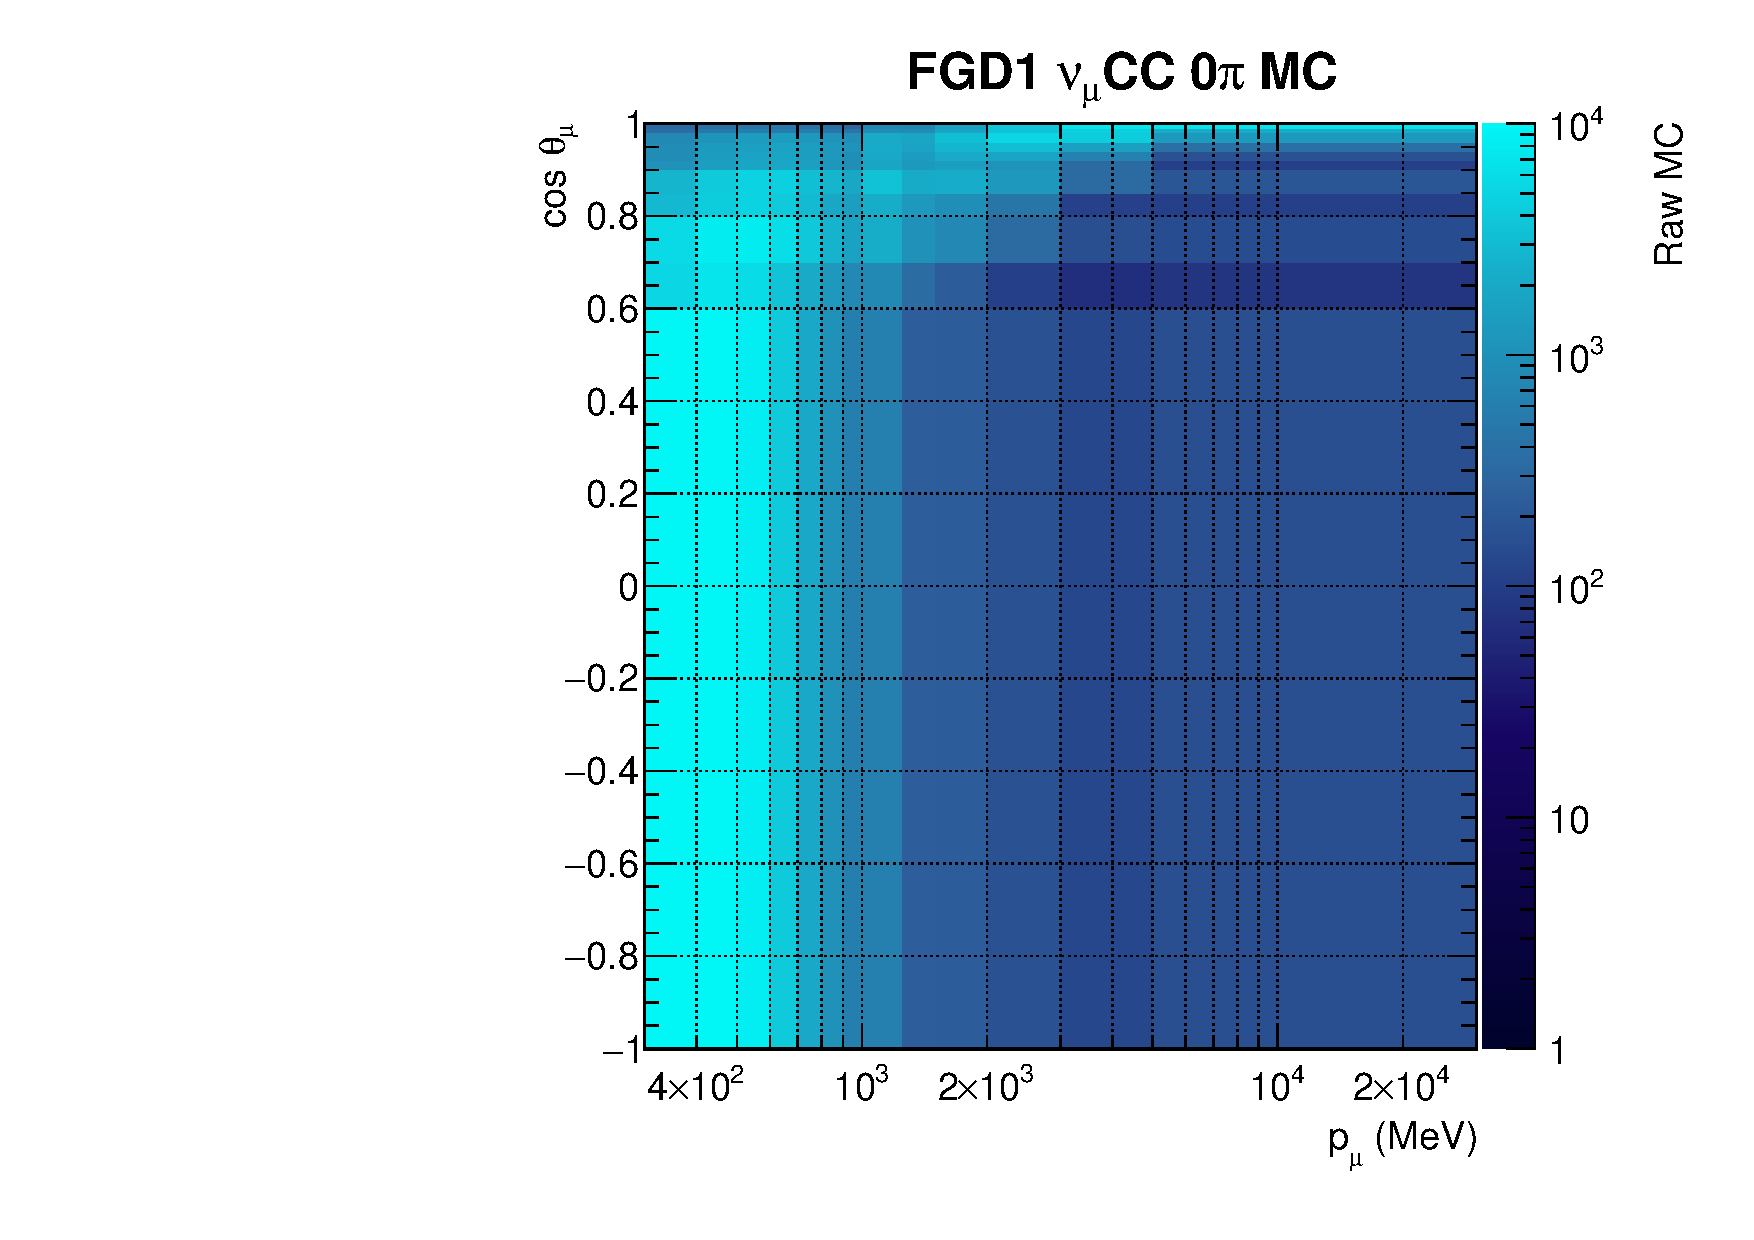
\includegraphics[width=\textwidth,page=1]{{figures/mach3/selection/2017b_nominal_withdebug_forthesis_noweightsapplied_onlyMCnom}}
	\end{subfigure}
	\begin{subfigure}[t]{0.32\textwidth}
		\includegraphics[width=\textwidth,page=2]{{figures/mach3/selection/2017b_nominal_withdebug_forthesis_noweightsapplied_onlyMCnom}}
	\end{subfigure}
	\begin{subfigure}[t]{0.32\textwidth}
		\includegraphics[width=\textwidth,page=3]{{figures/mach3/selection/2017b_nominal_withdebug_forthesis_noweightsapplied_onlyMCnom}}
	\end{subfigure}
	
	\begin{subfigure}[t]{0.32\textwidth}
		\includegraphics[width=\textwidth,page=4]{{figures/mach3/selection/2017b_nominal_withdebug_forthesis_noweightsapplied_onlyMCnom}}
	\end{subfigure}
	\begin{subfigure}[t]{0.32\textwidth}
		\includegraphics[width=\textwidth,page=5]{{figures/mach3/selection/2017b_nominal_withdebug_forthesis_noweightsapplied_onlyMCnom}}
	\end{subfigure}
	\begin{subfigure}[t]{0.32\textwidth}
		\includegraphics[width=\textwidth,page=6]{{figures/mach3/selection/2017b_nominal_withdebug_forthesis_noweightsapplied_onlyMCnom}}
	\end{subfigure}
	
	\begin{subfigure}[t]{0.24\textwidth}
		\includegraphics[width=\textwidth,page=7]{{figures/mach3/selection/2017b_nominal_withdebug_forthesis_noweightsapplied_onlyMCnom}}
	\end{subfigure}
	\begin{subfigure}[t]{0.24\textwidth}
		\includegraphics[width=\textwidth,page=8]{{figures/mach3/selection/2017b_nominal_withdebug_forthesis_noweightsapplied_onlyMCnom}}
	\end{subfigure}
	\begin{subfigure}[t]{0.24\textwidth}
		\includegraphics[width=\textwidth,page=9]{{figures/mach3/selection/2017b_nominal_withdebug_forthesis_noweightsapplied_onlyMCnom}}
	\end{subfigure}
	\begin{subfigure}[t]{0.24\textwidth}
		\includegraphics[width=\textwidth,page=10]{{figures/mach3/selection/2017b_nominal_withdebug_forthesis_noweightsapplied_onlyMCnom}}
	\end{subfigure}
	
	\begin{subfigure}[t]{0.24\textwidth}
		\includegraphics[width=\textwidth,page=11]{{figures/mach3/selection/2017b_nominal_withdebug_forthesis_noweightsapplied_onlyMCnom}}
	\end{subfigure}
	\begin{subfigure}[t]{0.24\textwidth}
		\includegraphics[width=\textwidth,page=12]{{figures/mach3/selection/2017b_nominal_withdebug_forthesis_noweightsapplied_onlyMCnom}}
	\end{subfigure}
	\begin{subfigure}[t]{0.24\textwidth}
		\includegraphics[width=\textwidth,page=13]{{figures/mach3/selection/2017b_nominal_withdebug_forthesis_noweightsapplied_onlyMCnom}}
	\end{subfigure}
	\begin{subfigure}[t]{0.24\textwidth}
		\includegraphics[width=\textwidth,page=14]{{figures/mach3/selection/2017b_nominal_withdebug_forthesis_noweightsapplied_onlyMCnom}}
	\end{subfigure}
	\caption{Raw Monte-Carlo event distributions for the 6CC\numu, 4CC\numubar and 4CC\numu in RHC, selections at ND280 in \pmu \cosmu. Red lines are regions of constant $Q^2_{\text{reco}}$ with fixed $E_\nu=0.6\text{ GeV}$}
	\label{fig:nominal_mc2d}
\end{figure}

\autoref{fig:nominal_mcpmu} and \autoref{fig:nominal_mccosmu} show the projections onto \pmu and \cosmu along with the composition by mode. \autoref{tab:nominal_mode} gives the mode breakdown of the histograms binned into 2D. The CC0$\pi$ samples have sizeable contributions from single pion interactions which is more than an effect from misreconstruction: in \autoref{fig:cc0pi_topology} the fraction of CC1$\pi$ topology events reconstructed as CC0$\pi$ was $\sim11\%$, whereas for the true interaction mode we have $\sim20\%$. This effect is almost entirely driven by final-state-interactions, in which nucleons and pions exit the nucleon-level interaction and are propagated through the nucleus with a probability of re-interaction with surrounding nucleons. A CC1$\pi^{0,+}$ interaction can see a pion absorbed, leaving only the outgoing muon, classifying it (correctly) as a CC0$\pi$ topology. This applies to all samples: feed-down occurs from pion absorption and feed-up occurs from inelastic nucleon or pion interactions, in which additional pions exit the nucleus. There is no effort to disentangle the effects of the fundamental interaction to that of final-state-interaction in this fit, as doing so is model dependent. In general, the selections perform well in separating the interaction models achieving above 65\% content for all samples. 

\autoref{fig:nominal_mcpmu} shows the fraction of single pion events in 0$\pi$ is highest at low momentum, reaching 50\% in the first bin. We also note the NC contribution is primarily focused in the 500-1000 MeV/c region for the 1$\pi$ and Other samples. It is also clear that the Other sample produces higher momentum muons, and mostly contains multi-$\pi$ and DIS events, as intended. 

Looking at the \cosmu projection in \autoref{fig:nominal_mccosmu}, the forward region of the CC0$\pi$ selection contains a large fraction of CC1$\pi$ events (50\%) and the highest amount of 2p2h. For the 1$\pi$ selection we note the CC coherent contribution almost exclusively in the most forward-going bin, as expected.
\begin{table}
	\centering
	\begin{tabular}{l | c c c c c c | c}
		\hline
		\hline
		Sample 			& CCQE & 2p2h & CC1$\pi^{\pm,0}$ 	& CC coh 	& CC multi-$\pi$ & CC DIS  	& NC \\
		\hline
		FGD1 0$\pi$	    & \textbf{58.0} & \textbf{10.1} & 19.6 & 0.3 & 4.2 & 4.6 & 3.1 \\
		FGD2 0$\pi$	    & \textbf{56.5} & \textbf{9.5}  & 21.3 & 0.3 & 4.6 & 4.7 & 3.1 \\
		\hline
		FGD1 1$\pi$	    & 5.6 & 0.9 & \textbf{50.8} & \textbf{2.8} & \textbf{17.7} & 16.1 & 6.0 \\
		FGD2 1$\pi$	    & 5.7 & 0.8 & \textbf{50.1} & \textbf{2.9} & \textbf{17.9} & 16.5 & 5.9 \\
		\hline
		FGD1 Other	    & 5.0 & 1.0 & 15.6 & 0.4 & \textbf{26.3} & \textbf{43.7} & 7.9 \\
		FGD2 Other	    & 5.3 & 1.1 & 16.3 & 0.4 & \textbf{25.8} & \textbf{43.6} & 7.6 \\
		\hline
		FGD1 1Trk	    	& \textbf{64.2} & \textbf{10.1} & 15.0 & 0.7 & 2.9 & 2.5 & 4.5 \\
		FGD2 1Trk	    	& \textbf{64.4} & \textbf{9.9} & 15.0 & 0.7 & 2.9 & 2.5 & 4.6 \\
		\hline
		FGD1 NTrk	    	& 7.8 & 2.7 & \textbf{29.3} & \textbf{3.4} & \textbf{20.3} & \textbf{26.0} & 10.5 \\ 
		FGD2 NTrk	  		& 8.7 & 2.6 & \textbf{29.0} & \textbf{3.3} & \textbf{20.5} & \textbf{25.4} & 10.5 \\
		\hline
		FGD1 1Trk   \numu 	& \textbf{44.5} & \textbf{8.5} & 25.4 & 0.9 & 7.2 & 6.2 & 7.5 \\
		FGD2 1Trk	\numu   & \textbf{43.8} & \textbf{8.3} & 25.5 & 0.8 & 7.7 & 6.6 & 7.2 \\
		FGD1 NTrk	\numu   & 12.6 & 3.1 & \textbf{29.3} & \textbf{1.8} & \textbf{20.9} & \textbf{25.6} & 6.6 \\ 
		\hline
		FGD2 NTrk	\numu   & 12.2 & 2.8 & \textbf{30.0} & \textbf{1.9} & \textbf{21.3} & \textbf{25.6} & 6.2 \\
		\hline
		\hline
	\end{tabular}
	\caption{Percentage mode breakdown for the binned nominal \textbf{unscaled} Monte-Carlo samples, \textbf{boldface} indicates interactions targeted by specific selections. The distributions are \textbf{not} bin-width normalised. Compare to \autoref{tab:nominal_mode_afterscale} for effect of weights}
	\label{tab:nominal_mode}
\end{table}

\begin{figure}[h]
	\begin{subfigure}[t]{0.2\textwidth}
		\includegraphics[width=\textwidth,page=15]{{figures/mach3/selection/2017b_nominal_withdebug_forthesis_noweightsapplied_onlyMCnom}}
	\end{subfigure}
	
	\begin{subfigure}[t]{0.32\textwidth}
		\includegraphics[width=\textwidth,page=16]{{figures/mach3/selection/2017b_nominal_withdebug_forthesis_noweightsapplied_onlyMCnom}}
	\end{subfigure}
	\begin{subfigure}[t]{0.32\textwidth}
		\includegraphics[width=\textwidth,page=18]{{figures/mach3/selection/2017b_nominal_withdebug_forthesis_noweightsapplied_onlyMCnom}}
	\end{subfigure}
	\begin{subfigure}[t]{0.32\textwidth}
		\includegraphics[width=\textwidth,page=20]{{figures/mach3/selection/2017b_nominal_withdebug_forthesis_noweightsapplied_onlyMCnom}}
	\end{subfigure}
	
	\begin{subfigure}[t]{0.32\textwidth}
		\includegraphics[width=\textwidth,page=22]{{figures/mach3/selection/2017b_nominal_withdebug_forthesis_noweightsapplied_onlyMCnom}}
	\end{subfigure}
	\begin{subfigure}[t]{0.32\textwidth}
		\includegraphics[width=\textwidth,page=24]{{figures/mach3/selection/2017b_nominal_withdebug_forthesis_noweightsapplied_onlyMCnom}}
	\end{subfigure}
	\begin{subfigure}[t]{0.32\textwidth}
		\includegraphics[width=\textwidth,page=26]{{figures/mach3/selection/2017b_nominal_withdebug_forthesis_noweightsapplied_onlyMCnom}}
	\end{subfigure}
	
	\begin{subfigure}[t]{0.24\textwidth}
		\includegraphics[width=\textwidth,page=28]{{figures/mach3/selection/2017b_nominal_withdebug_forthesis_noweightsapplied_onlyMCnom}}
	\end{subfigure}
	\begin{subfigure}[t]{0.24\textwidth}
		\includegraphics[width=\textwidth,page=30]{{figures/mach3/selection/2017b_nominal_withdebug_forthesis_noweightsapplied_onlyMCnom}}
	\end{subfigure}
	\begin{subfigure}[t]{0.24\textwidth}
		\includegraphics[width=\textwidth,page=32]{{figures/mach3/selection/2017b_nominal_withdebug_forthesis_noweightsapplied_onlyMCnom}}
	\end{subfigure}
	\begin{subfigure}[t]{0.24\textwidth}
		\includegraphics[width=\textwidth,page=34]{{figures/mach3/selection/2017b_nominal_withdebug_forthesis_noweightsapplied_onlyMCnom}}
	\end{subfigure}
	
	\begin{subfigure}[t]{0.24\textwidth}
		\includegraphics[width=\textwidth,page=36]{{figures/mach3/selection/2017b_nominal_withdebug_forthesis_noweightsapplied_onlyMCnom}}
	\end{subfigure}
	\begin{subfigure}[t]{0.24\textwidth}
		\includegraphics[width=\textwidth,page=38]{{figures/mach3/selection/2017b_nominal_withdebug_forthesis_noweightsapplied_onlyMCnom}}
	\end{subfigure}
	\begin{subfigure}[t]{0.24\textwidth}
		\includegraphics[width=\textwidth,page=40]{{figures/mach3/selection/2017b_nominal_withdebug_forthesis_noweightsapplied_onlyMCnom}}
	\end{subfigure}
	\begin{subfigure}[t]{0.24\textwidth}
		\includegraphics[width=\textwidth,page=42]{{figures/mach3/selection/2017b_nominal_withdebug_forthesis_noweightsapplied_onlyMCnom}}
	\end{subfigure}
	\caption{Raw Monte-Carlo event distributions for the 6CC\numu, 4CC\numubar and 4CC\numu in RHC, selections at ND280 projected onto \pmu and bin-width normalised}
	\label{fig:nominal_mcpmu}
\end{figure}

\begin{figure}[h]
	\begin{subfigure}[t]{0.32\textwidth}
		\includegraphics[width=\textwidth,page=17]{{figures/mach3/selection/2017b_nominal_withdebug_forthesis_noweightsapplied_onlyMCnom}}
	\end{subfigure}
	\begin{subfigure}[t]{0.32\textwidth}
		\includegraphics[width=\textwidth,page=19]{{figures/mach3/selection/2017b_nominal_withdebug_forthesis_noweightsapplied_onlyMCnom}}
	\end{subfigure}
	\begin{subfigure}[t]{0.32\textwidth}
		\includegraphics[width=\textwidth,page=21]{{figures/mach3/selection/2017b_nominal_withdebug_forthesis_noweightsapplied_onlyMCnom}}
	\end{subfigure}
	
	\begin{subfigure}[t]{0.32\textwidth}
		\includegraphics[width=\textwidth,page=23]{{figures/mach3/selection/2017b_nominal_withdebug_forthesis_noweightsapplied_onlyMCnom}}
	\end{subfigure}
	\begin{subfigure}[t]{0.32\textwidth}
		\includegraphics[width=\textwidth,page=25]{{figures/mach3/selection/2017b_nominal_withdebug_forthesis_noweightsapplied_onlyMCnom}}
	\end{subfigure}
	\begin{subfigure}[t]{0.32\textwidth}
		\includegraphics[width=\textwidth,page=27]{{figures/mach3/selection/2017b_nominal_withdebug_forthesis_noweightsapplied_onlyMCnom}}
	\end{subfigure}
	
	\begin{subfigure}[t]{0.24\textwidth}
		\includegraphics[width=\textwidth,page=29]{{figures/mach3/selection/2017b_nominal_withdebug_forthesis_noweightsapplied_onlyMCnom}}
	\end{subfigure}
	\begin{subfigure}[t]{0.24\textwidth}
		\includegraphics[width=\textwidth,page=31]{{figures/mach3/selection/2017b_nominal_withdebug_forthesis_noweightsapplied_onlyMCnom}}
	\end{subfigure}
	\begin{subfigure}[t]{0.24\textwidth}
		\includegraphics[width=\textwidth,page=33]{{figures/mach3/selection/2017b_nominal_withdebug_forthesis_noweightsapplied_onlyMCnom}}
	\end{subfigure}
	\begin{subfigure}[t]{0.24\textwidth}
		\includegraphics[width=\textwidth,page=35]{{figures/mach3/selection/2017b_nominal_withdebug_forthesis_noweightsapplied_onlyMCnom}}
	\end{subfigure}
	
	\begin{subfigure}[t]{0.24\textwidth}
		\includegraphics[width=\textwidth,page=37]{{figures/mach3/selection/2017b_nominal_withdebug_forthesis_noweightsapplied_onlyMCnom}}
	\end{subfigure}
	\begin{subfigure}[t]{0.24\textwidth}
		\includegraphics[width=\textwidth,page=39]{{figures/mach3/selection/2017b_nominal_withdebug_forthesis_noweightsapplied_onlyMCnom}}
	\end{subfigure}
	\begin{subfigure}[t]{0.24\textwidth}
		\includegraphics[width=\textwidth,page=41]{{figures/mach3/selection/2017b_nominal_withdebug_forthesis_noweightsapplied_onlyMCnom}}
	\end{subfigure}
	\begin{subfigure}[t]{0.24\textwidth}
		\includegraphics[width=\textwidth,page=43]{{figures/mach3/selection/2017b_nominal_withdebug_forthesis_noweightsapplied_onlyMCnom}}
	\end{subfigure}
	\caption{Raw Monte-Carlo event distributions for the 6CC\numu, 4CC\numubar and 4CC\numu in RHC, selections at ND280 projected onto \cosmu and bin-width normalised}
	\label{fig:nominal_mccosmu}
\end{figure}
\fi
